The constant $c_s$ model was chosen as the model to test PTtools with,
as the model is the next logical extension of the bag model,
and there is some reference data available from \cites{giese_2020}{giese_2021}.
Figure \ref{fig:fluid_profiles} demonstrates solutions for three different wall speeds $v_\text{wall}$ and two different $\alpha_n$.
% These are not the same as the values \cite[fig. 10]{hindmarsh_gw_pt_2019}.
Instead of using only the bag model $c_{s,s}^2 = c_{s,b}^2 = \frac{1}{3}$,
each plot has four curves, each corresponding to a different combination of the sound speeds
$c_{s,s}^2 \in \{ \frac{1}{3}, \frac{1}{4} \}, c_{s,b}^2 \in \{ \frac{1}{3}, \frac{1}{4} \}$.
The corresponding gravitational wave spectra are plotted in \ref{fig:gw_spectra}.
Converting these to the frequencies today results in the figure \ref{fig:omgw0},
which also contains the LISA instrument noise spectrum as a reference.

\begin{figure}[ht!]
\centering
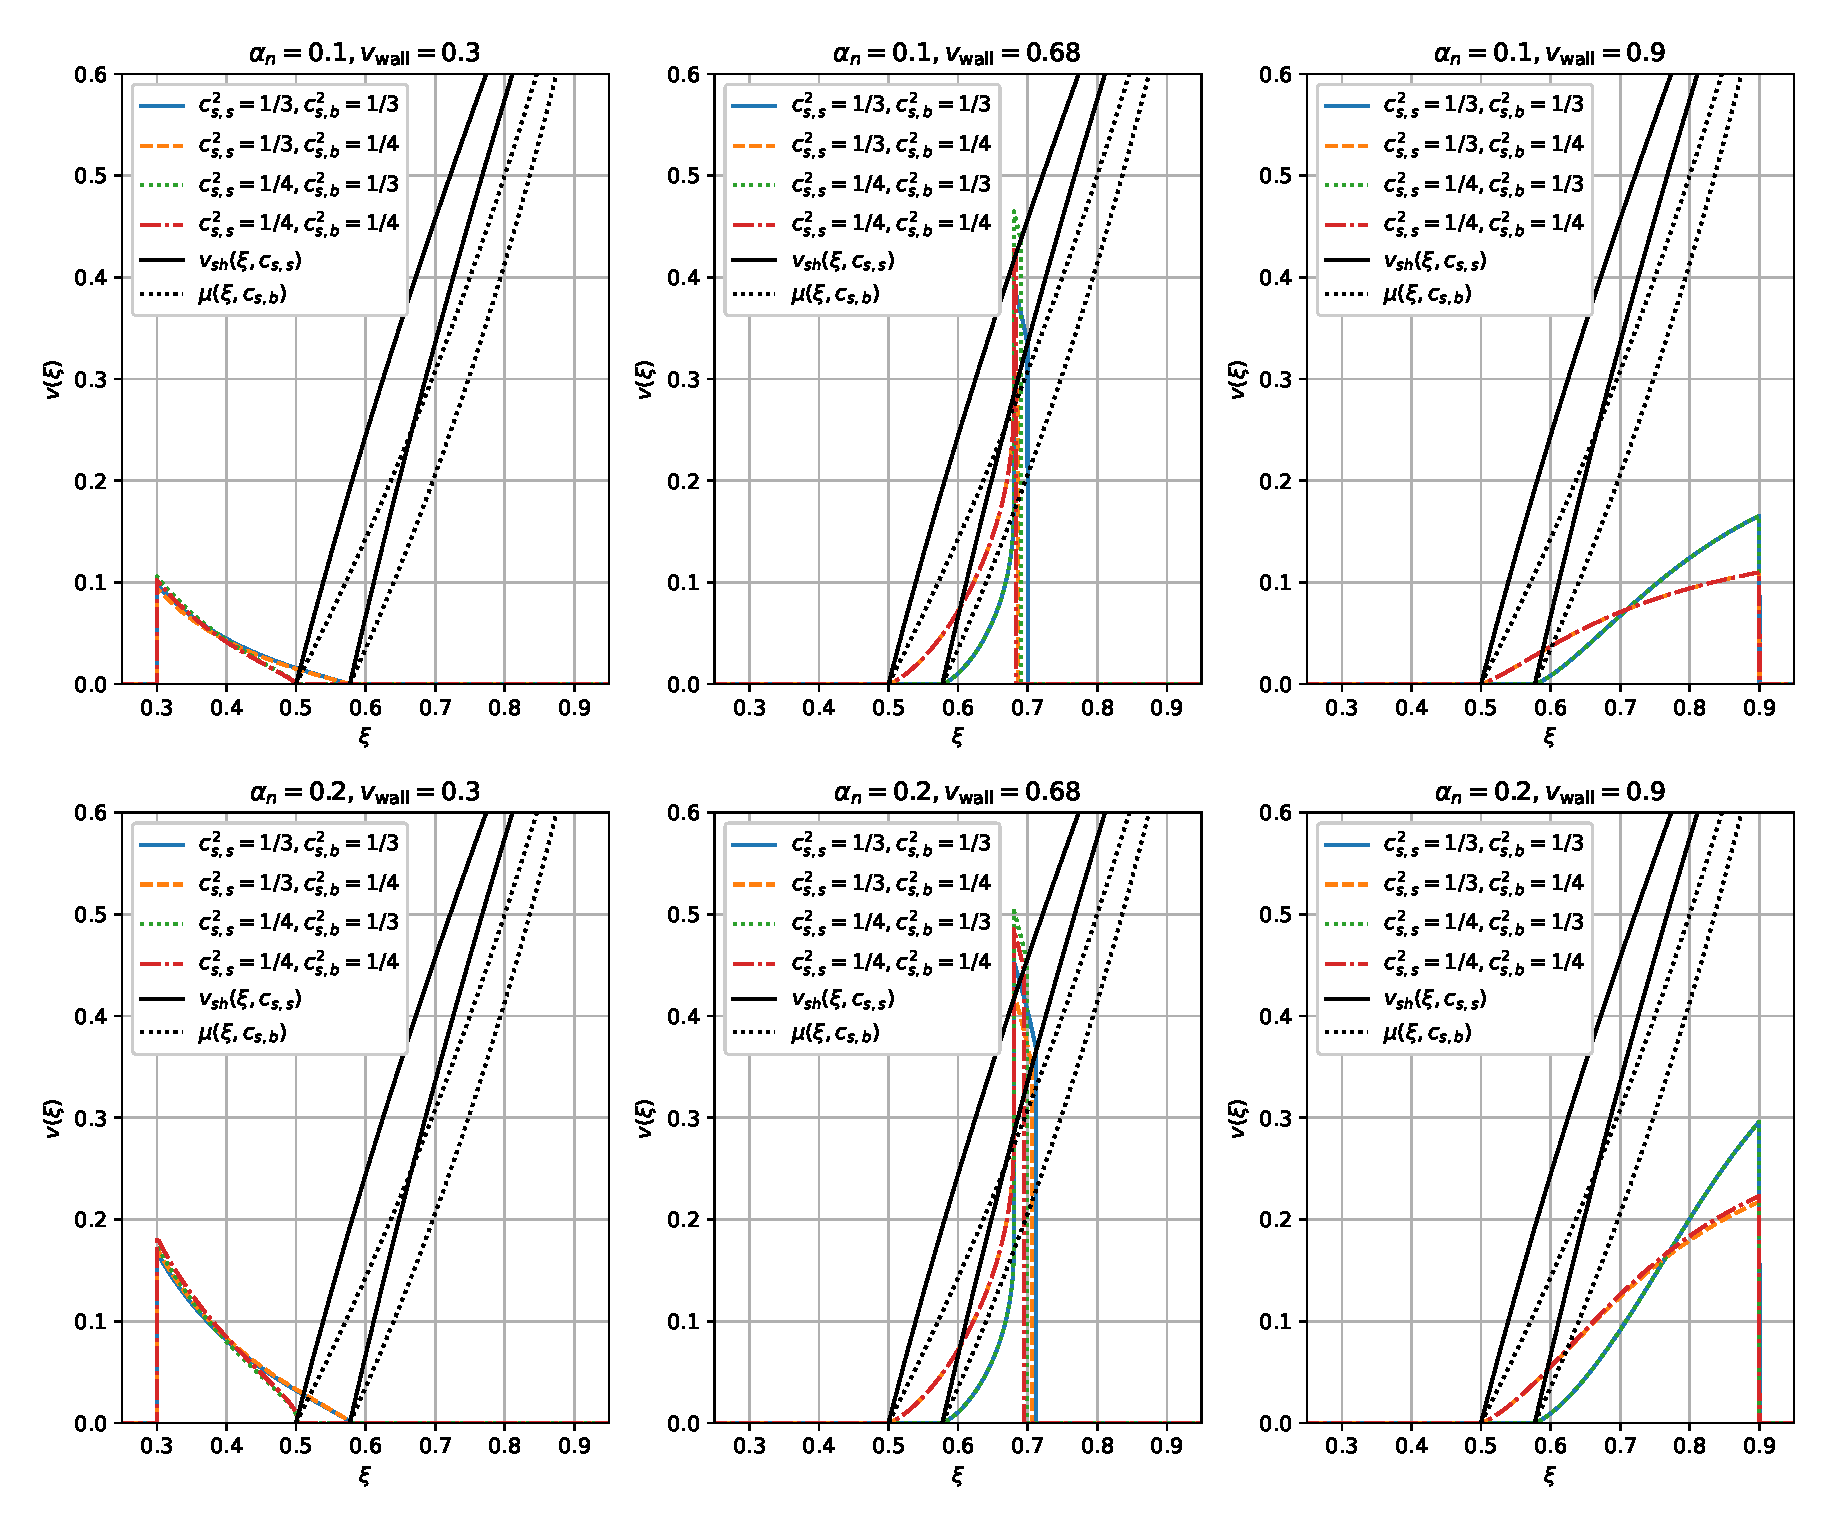
\includegraphics[width=\textwidth]{../pttools/examples/fig/const_cs_gw_v.eps}
\caption{Self-similar fluid profiles}
\label{fig:fluid_profiles}
\end{figure}

\begin{figure}[ht!]
\centering
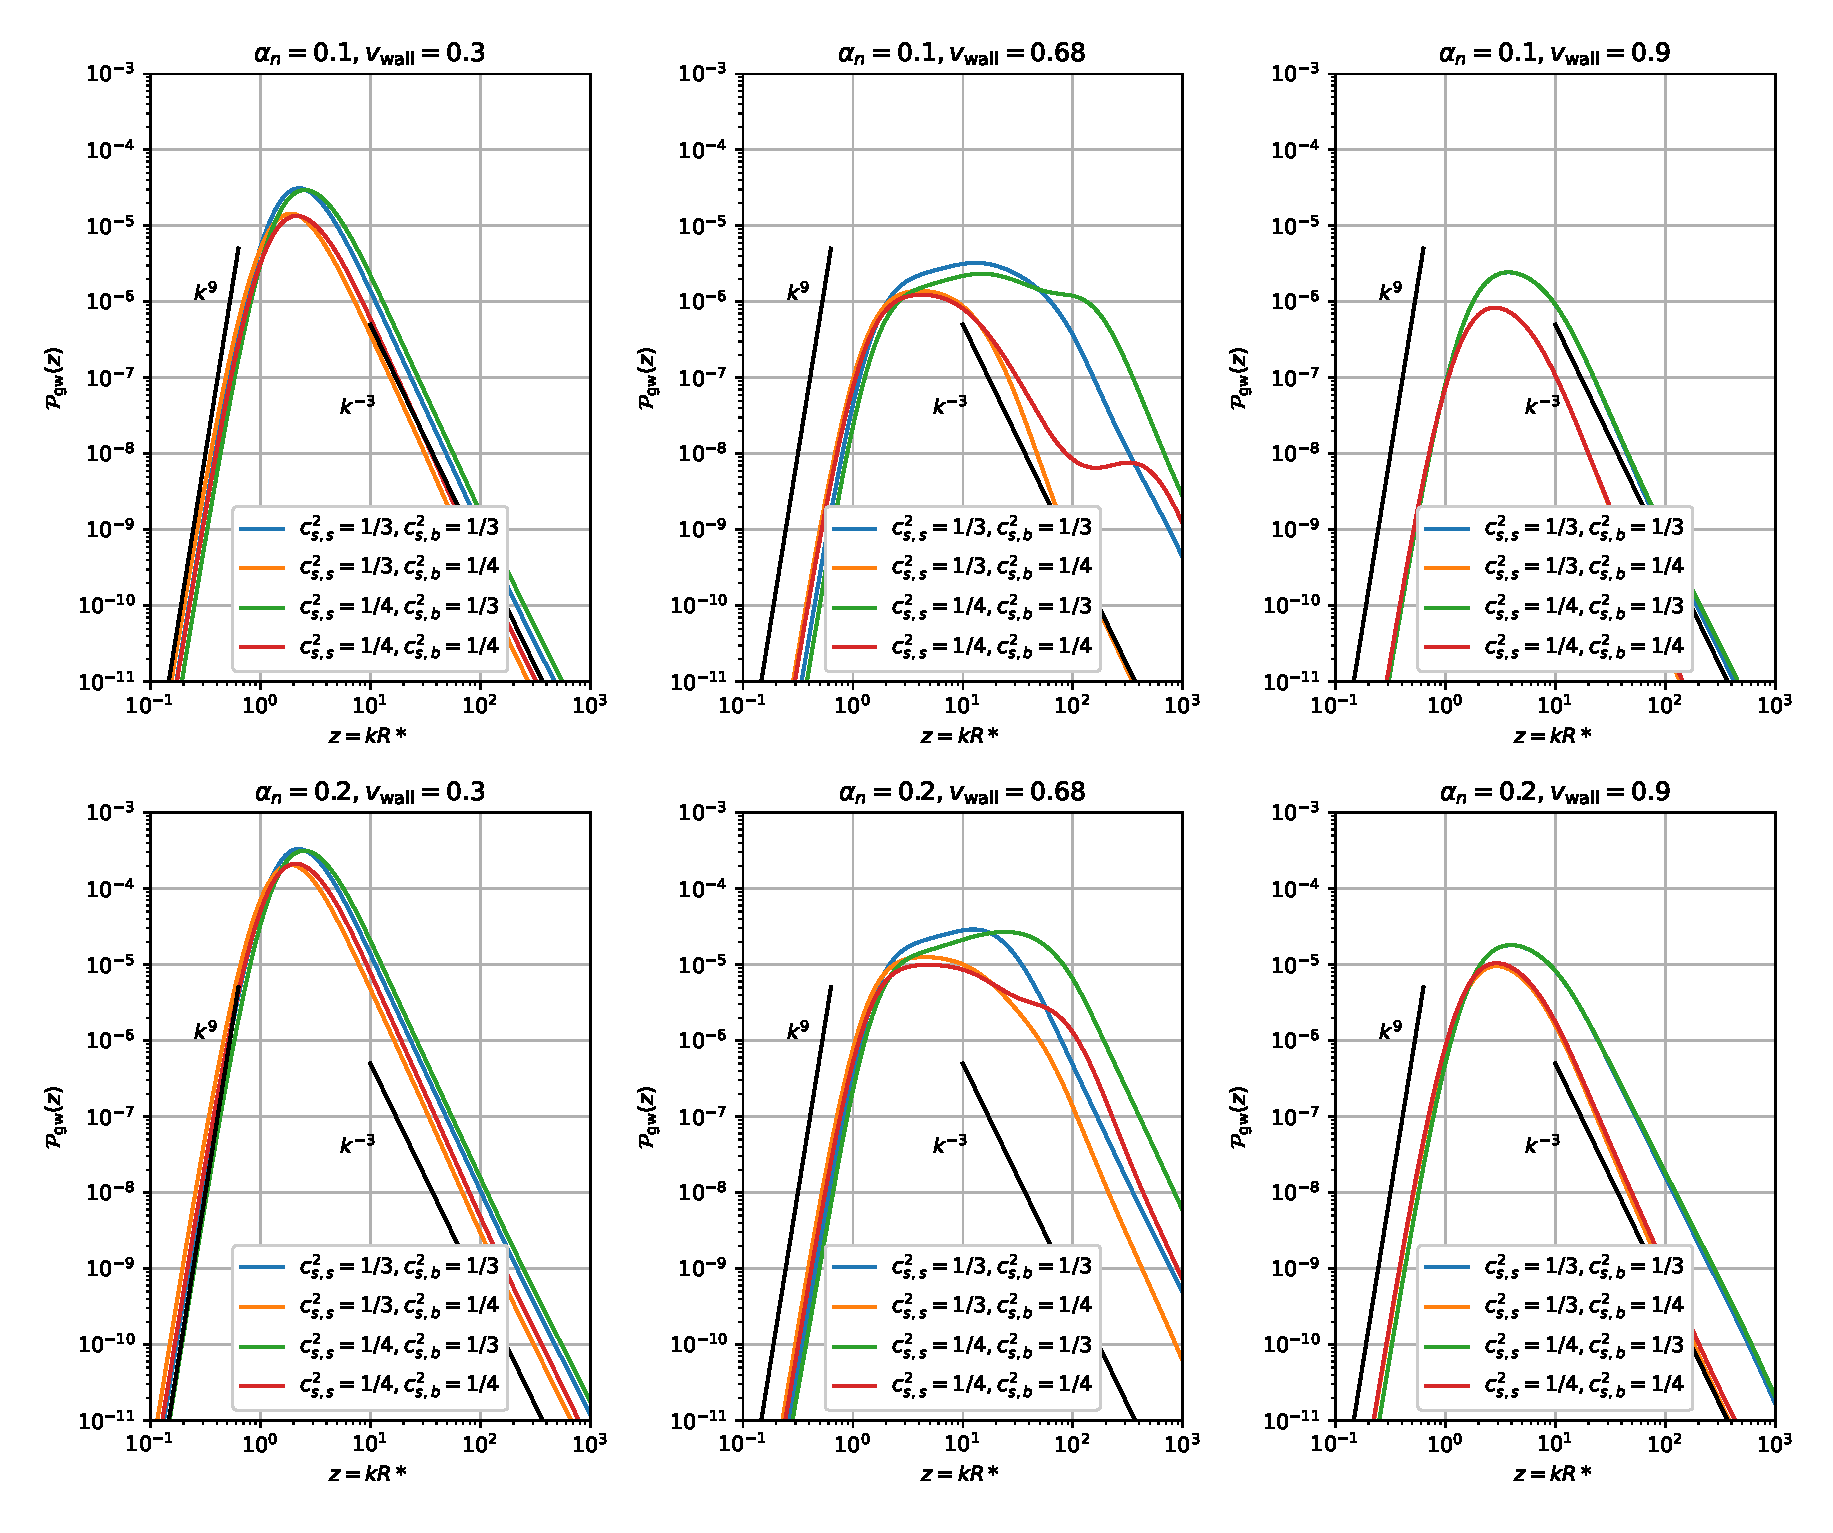
\includegraphics[width=\textwidth]{../pttools/examples/fig/const_cs_gw.eps}
\caption{Gravitational wave power spectra}
\label{fig:gw_spectra}
\end{figure}

\begin{figure}[ht!]
\centering
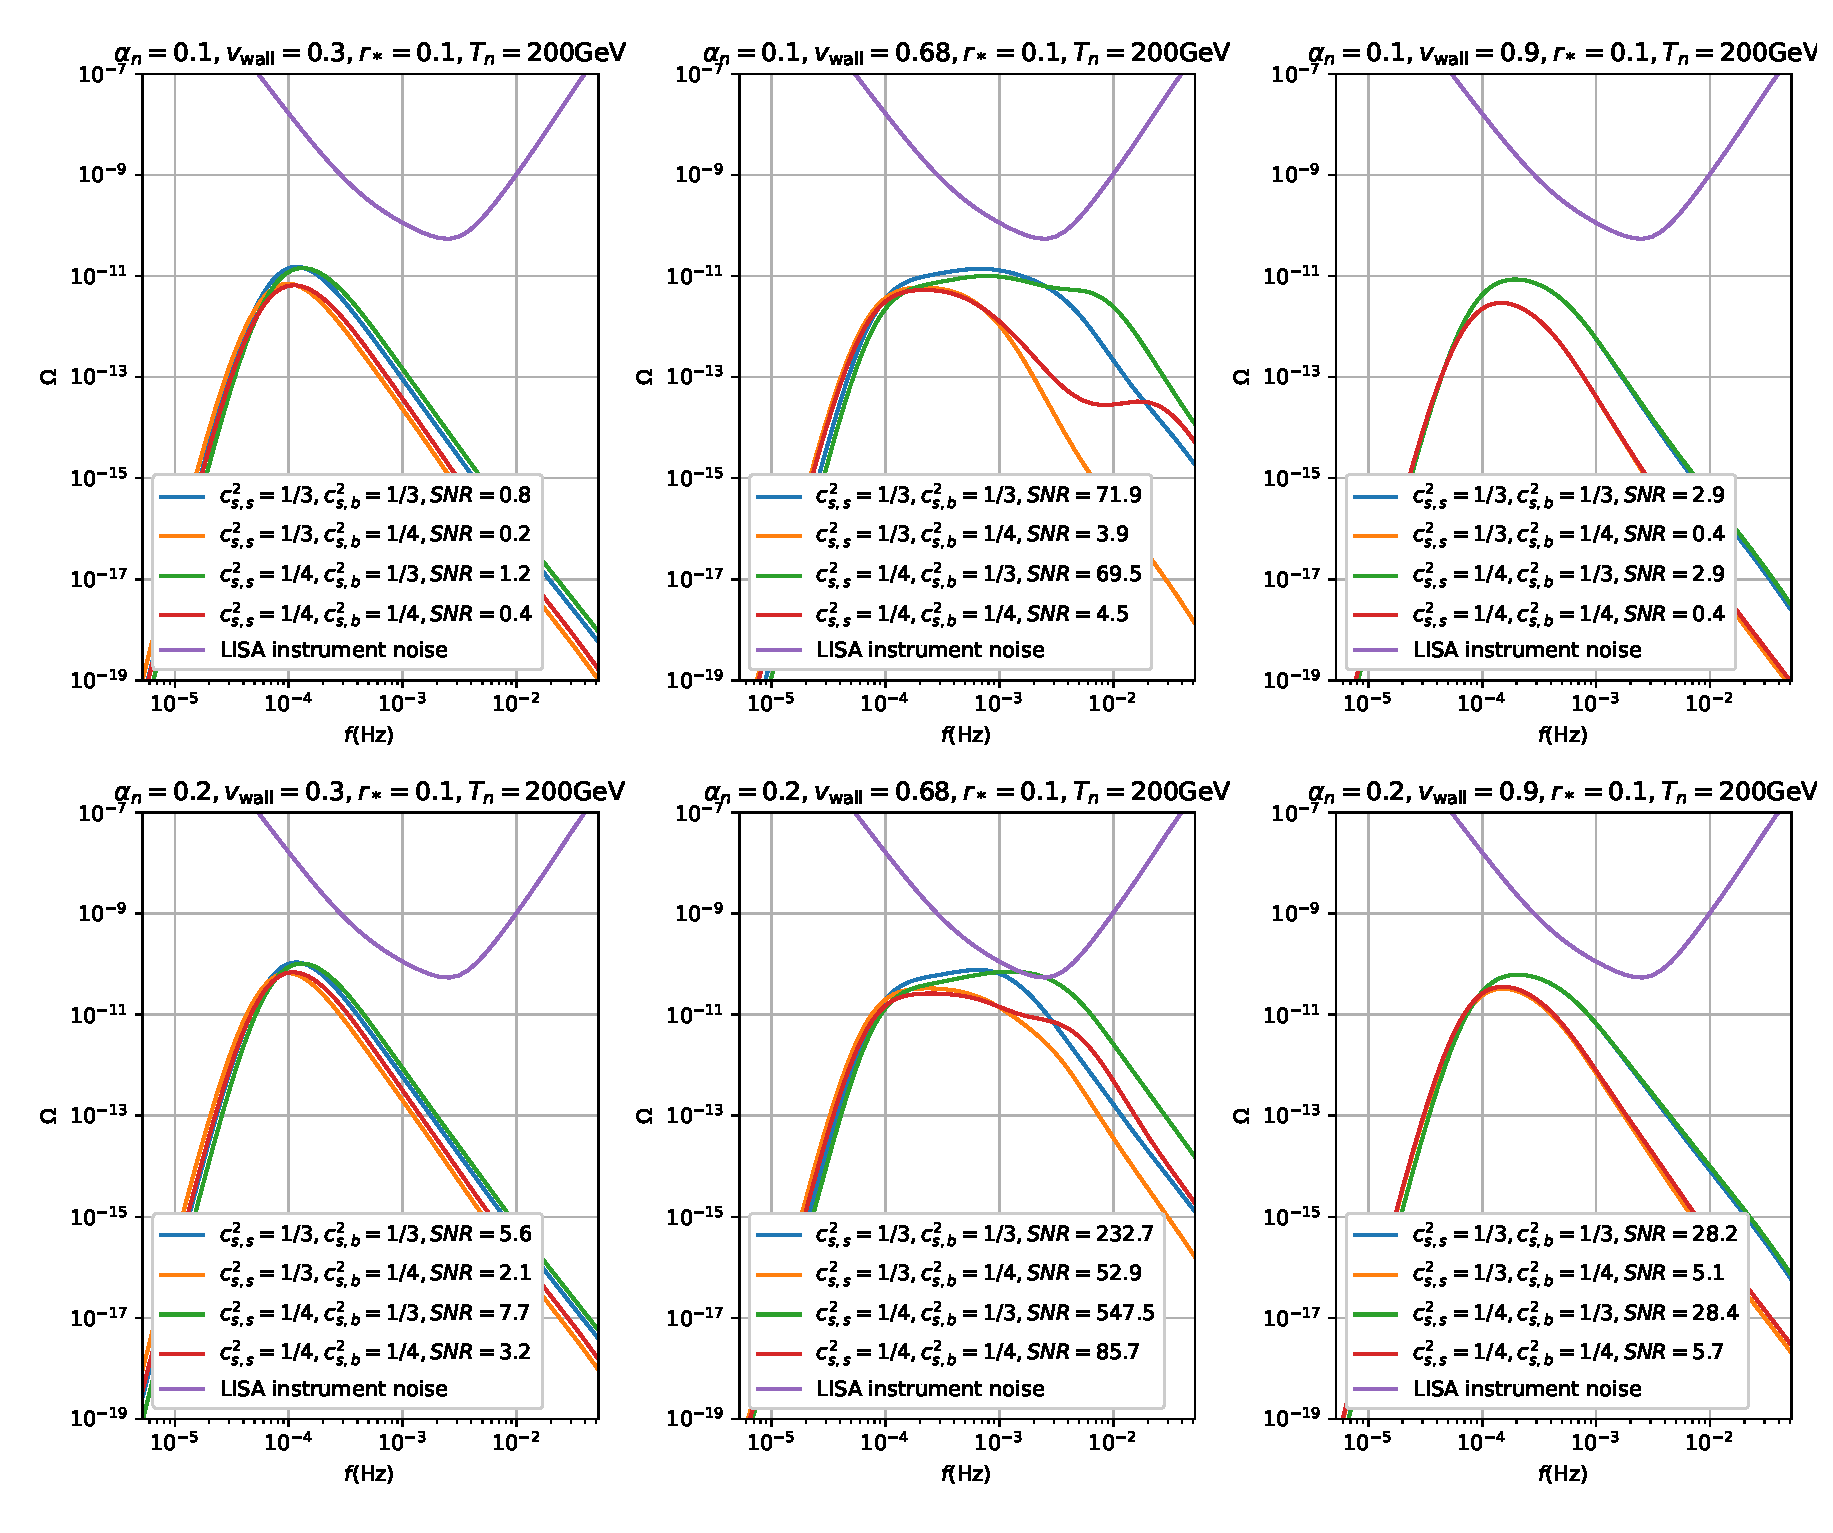
\includegraphics[width=\textwidth]{../pttools/examples/fig/const_cs_gw_omgw0.eps}
\caption{Gravitational wave power spectra today $\Omega_{gw,0}$}
\label{fig:omgw0}
\end{figure}

These figures demonstrate that the sound speed can have a profound effect on the resulting gravitational wave spectrum.
To understand how the sound speed affects the gravitational wave spectrum,
we have to first study the fluid shells of figure \ref{fig:fluid_profiles}.
There are two curves that constrain the shape of the fluid shells.
The solid black curves are the shock velocities $v_{sh}(\xi,c_{s,s})$ that are determined by $c_{s,s}$.
In general the shock velocity is also dependent on $w$, since $c_s = c_s(w,\phi)$,
but in the constant sound speed model the sound speed is independent of the enthalpy,
as it's a constant for each phase.
Therefore we can plot the shock velocities as curves in the 2D plots instead of having to plot them as surfaces as functions of $(\xi,w)$ in a 3D plot.
The dotted black curves are the $\mu(\xi,c_{s,b})$ curves of eq. \eqref{eq:mu} that constrain the maximum fluid velocity inside the bubble.
They are dependent on the choice of $c_{s,b}$.
The $v_{sh}$ curves encounter $v=0$ at $\xi = c_{s,s}$ and the $\mu$ curves at $\xi = c_{s,b}$.

For all solution types, adjusting either of the sound speeds affects the degrees of freedom and therefore the pressure $p$ and enthalpy $w$ for that phase.
This affects the solution of the bubble wall junction conditions of eq. \eqref{eq:junction_condition_1}, \eqref{eq:junction_condition_2} and therefore $v(\xi_\text{wall})$,
which is also the peak of the fluid velocity profile.
This effect can be seen at the top-left figure, where all four fluid shells have different $v(\xi_\text{wall})$.
The change caused by adjusting the sound speed is the most profound for deflagrations when $c_{s,s}$ is decreased below $v_\text{wall}$, as it causes them to become hybrids, and vice versa.
Similarly changing $c_{s,b}$ so that the Chapman-Jouguet speed of \eqref{eq:chapman_jouguet} is decreased below $v_\text{wall}$ converts a hybrid to a detonation, and vice versa.
This can be seen at the top-right figure.

For deflagrations and hybrids, adjusting $c_{s,s}$ affects the location of the shock and therefore the thickness of the fluid shell.
It also affects the ODE group of eq. \eqref{eq:hydro_param1}, \eqref{eq:hydro_param2}, \eqref{eq:hydro_param3} and therefore the shape of the fluid shell in front of the bubble wall.
These effects can be seen at the top-left and bottom-left figures, where the curves with the same $c_{s,s}$ are grouped together.
Correspondingly for hybrids, adjusting $c_{s,b}$ affects $\mu(\xi_\text{wall},c_{s,b})$,
which is the point from which the integration of the detonation-like part of the fluid shell starts.
This can be seen in the two figures at the middle, where the detonation-like tails of the curves with the same $c_{s,b}$ are grouped together.
And for both detonations and hybrids, adjusting $c_{s,b}$ affects the shape of the fluid shell behind the wall.

These differences in the shapes of the fluid shells carry over to the gravitational wave spectra of fig. \ref{fig:gw_spectra} and eventually of the gravitational wave spectra today in fig. \ref{fig:omgw0}.
The sine transformation of eq. \todo{Add equation reference} that converts the fluid shells of fig. \ref{fig:fluid_profiles} to the gravitational wave spectra of \ref{fig:gw_spectra} has the same basic properties as a Fourier transform.
Therefore by comparing the fluid velocity profiles and the gravitational wave spectra we can identify a few general correlations.
The thinner the fluid shell is, the broader the gravitational wave spectrum.
And the higher the fluid velocities are in the fluid shell, the higher is the intensity of the gravitational waves.
Thin shells also have more of the higher frequencies.
These effects can be seen in the case of thin hybrids of the middle and right figures.
Hybrids consist of two sections with significantly differing characteristics.
Therefore the hybrids and especially the thin hybrids with high fluid velocities in front of the wall have a gravitational wave spectrum with two distinct contributions.
This results in a significantly higher gravitational wave spectrum in the higher frequencies resulting in a significantly higher signal-to-noise ratio (SNR),
which distinguishes them from the detonations and deflagrations.
However, regarding hybrids and especially these thin hybrids
it should be noted that the hybrid solutions are very finely tuned, and may not exist in a real fluid.
\cite[p. 5]{gowling_lisa_2021}
Outside the region of the peak, the gravitational wave spectra follow a $k^9$ power law at low $z$,
and $k^{-3}$ at high $z$.

To test the precision and reliability of the results provided by PTtools,
we compared to the results in \cite[fig. 2]{giese_2021},
resulting in figure \ref{fig:kappa_giese}.
It should be noted that the article uses $\kappa_{\bar{\theta}_n}$ of eq. \eqref{eq:kappa_thetabar_n},
which differs from the $\kappa$ defined in eq. \eqref{eq:kappa_omega}.
The colors from blue to gray correspond to $\alpha = 0.01, 0.03, 0.1, 0.3, 1, 3$.
The figures on the left have $\alpha = \alpha_{\bar{\theta}_n}$
and the figures on the right have $\alpha = \alpha_n$.
For each color, the upper line has $c_{s,b}^2 = \frac{1}{3}$ and the lower line $c_{s,b}^2 = \frac{1}{4}$.
The solid lines correspond to $c_{s,s}^2 = \frac{1}{3}$ and the dashed lines correspond to $c_{s,s}^2 = \frac{1}{4}$.

\begin{figure}[ht!]
\centering
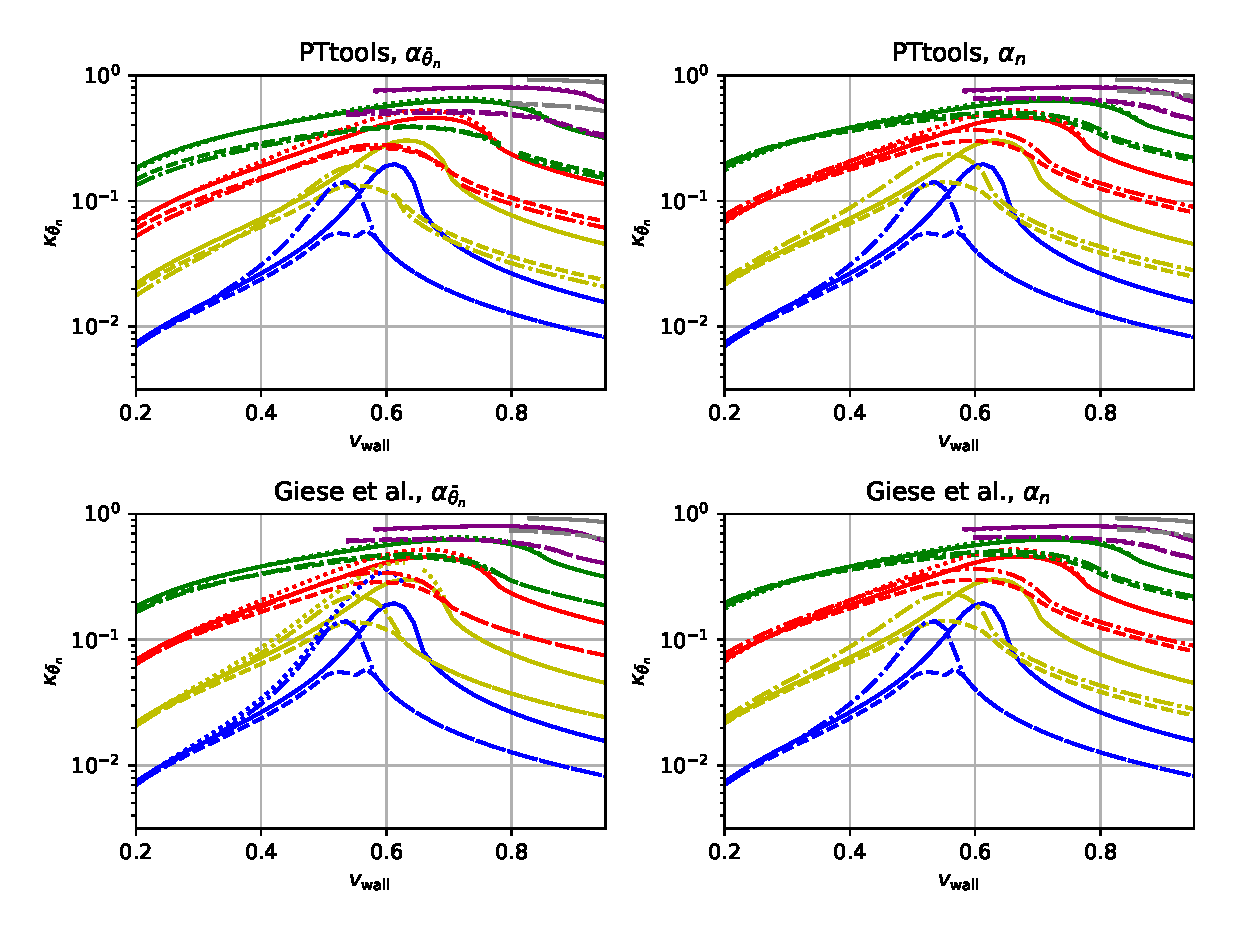
\includegraphics[width=\textwidth]{../pttools/examples/fig/giese_lisa_fig2.eps}
\caption{Comparison of $\kappa_{\bar{\theta}_n}$ values by \cite[fig. 2]{giese_2021} and PTtools}
\label{fig:kappa_giese}
\end{figure}

Comparing the results proved out to be challenging for several reasons.
PTtools operates natively with $\alpha_n$, whereas the Giese code uses $\alpha_{\bar{\theta}_n}$.
Therefore to compare the results, one has to be converted to the other before giving the value to the corresponding code.
There is no known analytical solution for this conversion, and therefore it has to be done numerically.
This may introduce a slight numerical error in $\alpha$ for either one of the solvers.

The Giese code does not check that the input parameter values allow for a physical solution,
and therefore the the parameter region chosen for the figure contains unphysical sections.
For the sound speeds $c_{s,s}^2 = \frac{1}{4}, c_{s,b}^2 = \frac{1}{3}$ the $\alpha = 0.01, 0.03$ values turned out to be below the theoretical minimum
required for a critical temperature to exist.
Therefore the upper dashed blue $\alpha = 0.01$ and yellow $\alpha = 0.03$ lines are missing.
The Giese figures have these solutions, even though they are unphysical.

Nearly all the PTtools figures have a single gap.
This is caused by that particular $\xi_\text{wall}$ value being so near the Chapman-Jouguet speed $v_{CJ}$ of the hybrid-detonation boundary
that the thickness of the fluid shell in front of the is comparable to the minimum step of the ODE solver
and the search step of the shooting algorithm that adjusts the starting point.
This results in the solver being unable to find a solution.
However, it should be noted that this is a pathological special case for the fluid shell solver,
and that for the vast majority of the $(v_\text{wall}, \alpha_n)$ parameter space it works reliably.
Work is being done to improve the solver to work beyond these issues.
The Giese code avoids these issues by using analytical shortcuts specific to the constant sound speed model,
whereas the PTtools solver is intentionally designed to be general so that it will work with more complex models as well.
However, there are also regions in which even the Giese code, as it is shown in an appendix of the article, is not able to find a solution.
Interestingly this curve is present in the figure of the article.
Possible causes include that the code used to generate the figure was different than the one in the appendix,
or that some of the underlying libraries has changed over time.
This is demonstrated by the lack of the dashed blue $\alpha_n = 0.01, c_{s,s}^2 = \frac{1}{4}, c_{s,b}^2 = \frac{1}{3}$ in the bottom-right figure,
and the abrupt end of the same curve in the bottom-left $\alpha_{\bar{\theta}_n}$.

It is also possible that the various validity checks don't capture all the issues at this boundary,
resulting in a slightly wrong result.
This is demonstrated by the solid green $\alpha_n = 0.3, c_{s,s}^2 = \frac{1}{4}, c_{s,b} = \frac{1}{4}$ curve in the top-right figure,
where one of the points deviates from the curve.
These issues continue to be under investigation.

There are also slight differences in the numerical values produced by the solvers.
These are the most visible for the $\alpha_n$ figures, where for high $\xi_\text{wall}$ the effect on changing $c_{s,s}$ has the opposite effect on $\kappa$.
This too continues to be under investigation.
Given that \cites{giese_2020}{giese_2021} are the only known references known by the author regarding the effects of changing the sound speed on the fluid shell profile,
the numerical imprecisions can be either in PTtools or the Giese code, or both.
The development of the code continues.
